\documentclass[11pt]{article}
\usepackage{geometry}
 \geometry{
 letterpaper,
 left=1in,
 right=1in,
 top=1in,
 bottom=1in
 }
\usepackage[utf8]{inputenc}

\usepackage[super,sort&compress,numbers]{natbib}
\bibliographystyle{naturemag}
%\bibliographystyle{plainnat} %abbrv, acm, alpha, apalike, ieeetr, plain, siam, unsrt
\usepackage{url}
\urlstyle{same}
\usepackage{color}
\usepackage{graphicx}
\usepackage{longtable}
\usepackage{setspace}
\usepackage[skip=10pt, indent=20pt]{parskip}
\usepackage{changepage}
\usepackage[normalem]{ulem}
\usepackage{arydshln}
\usepackage[font=small] {caption}
\usepackage{subcaption}
\usepackage{chngcntr}
\usepackage{wrapfig}
\usepackage{sidecap}
\sidecaptionvpos{figure}{c} 
\usepackage{amsmath,amssymb,amsthm} % AMS styles for extra equation formatting
\usepackage{cleveref}
\renewcommand\thesection{\Roman{section}}
\renewcommand\thesubsection{\thesection.\arabic{subsection}}
\begin{document}

\section{Invasion of a Disease on a Landscape}

\section{Derivation}

Consider a gridded 2D space where the probability that an individual is located in a cell is given by $w_{i,j}$, where for a given cell, the value $w_{i,j}$ is computed as 

\begin{equation}
    w_{i,j} = \text{Max}(0, f(T_{i,j}, R_{i,j}))
\end{equation}

where $f(T_{i,j}, R_{i,j})$ is the function defining the suitability of patch $i,j$ based on (something we need to define more clearly):

\begin{equation}
    f(T_{i,j}, R_{i,j}) = \frac{I_{\text{max}}(T_{i,j} R_{i,j})}{R_{i,j} + R_{\text{half}}} - m(T_{i,j}),
\end{equation}
with $m(T)$ being a respiration term of the organism, and $I_{\text{max}(T)}$ is the maximum uptake rate, where $m(T) = m_a e^{m_b \times T} + m_c$ and $I_{\text{max}}(T) = e^{-(T - T_I)^2 / \gamma}$ with $m$ being an approximated exponential version of the Boltzmann-Arrhenius relationship. Here $T_I$ is the optimal temperature value and $\gamma$ determines the breadth of the response. This value is dependent on each cell, where $T_{i,j}$ is the temperature value at $i,j$ and $R_{i,j}$ is the inflow supply of some resource for the organism choosing it's location \Cref{fig:t-s-wij-grid}. The values for a given cell of $T$ and $S$ are drawn from: 

\begin{align} \label{eq:s-t}
    T_{i,j} \sim \mathcal{N}(\mu_T, \sigma_T) \\
    R_{i,j} \sim \mathcal{N}(\mu_R, \sigma_R)
\end{align}

which produce the distributions shown in \Cref{fig:t-s-wij-pdfs}:

\begin{figure}[!hpt]
    \centering
    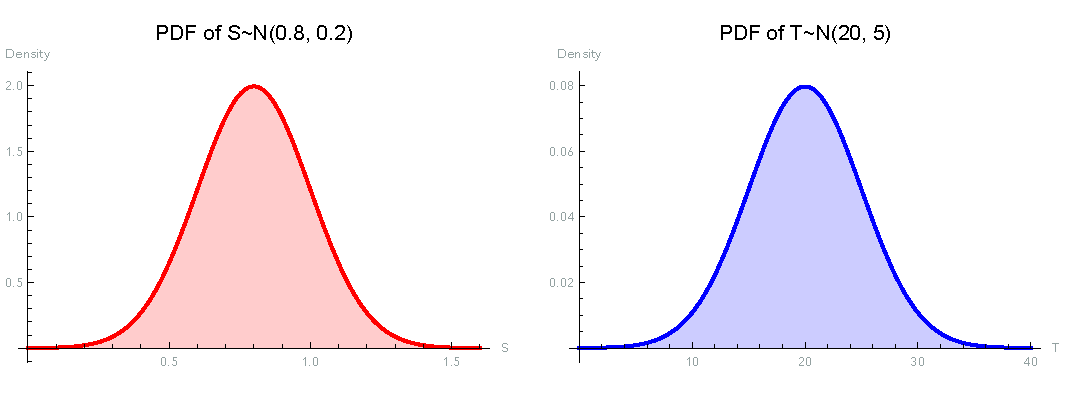
\includegraphics[width=0.9\linewidth]{figs/temp-supply-wij-pdfs.pdf}
    \caption{Temperature values, supply values, drawn from distributions given by \Cref{eq:s-t}.}
    \label{fig:t-s-wij-pdfs}
\end{figure}

and for convenience, we set $m_a = 0.01, m_b = 0.1, m_c = 0.05, T_I = 20, R_{\text{half}} = 0.5, \mu_T = 20, \sigma_ T = 5, \alpha_S = 1.2, $ and $\beta_S = 1$. 

Since these are probabilities it must be true that 
\begin{equation}
\sum_i \sum_j w_{i,j}=1.
\end{equation}

\begin{figure}[!hpt]
    \centering
    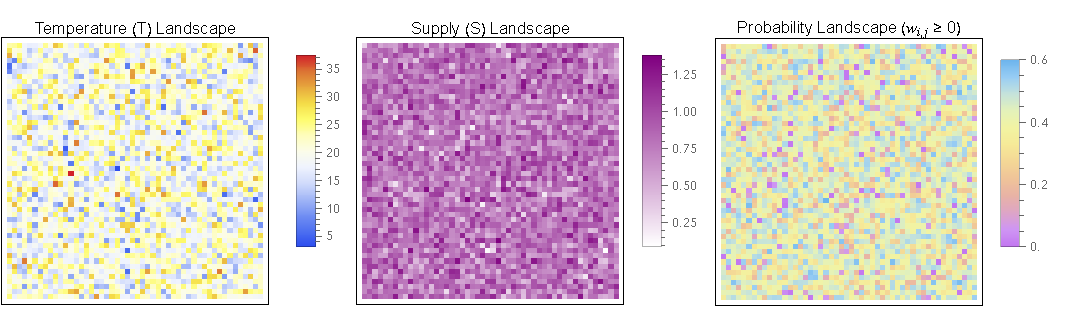
\includegraphics[width=0.9\linewidth]{figs/temp-supply-probability-landscape.pdf}
    \caption{Temperature values, supply values, and subsequent probabilities of a given organism being located in a given cell.}
    \label{fig:t-s-wij-grid}
\end{figure}

If there are $S$ susceptible individuals in the population that assort randomly across space according to the probabilities $w_{i,j}$ and $I=1$ infected individual, we want to know the probability that the disease will spread. From a purely contact perspective, this is given by the probability that the infected individual occupies a location that also has at least one susceptible individual. 

\subsection{Determining the probability that at least one $S$ is located in a cell $i,j$}

The probability that patch $i,j$ has zero susceptible individuals is $P(S_{i,j}=0)=(1-w_{i,j})^S$, where $S$ is the number of susceptible individuals on the landscape. Thus, the probability that at least one patch at location $i,j$ has at least one susceptible individual is given by:  
\begin{align}
P(s_{i,j} \geq 1) &=1-P(s_{i,j}=0) \\
&=P(s_{i,j}=1)+P(s_{i,j}=2)+P(s_{i,j}=3)+ ... +P(s_{i,j}=S)
\end{align}
Each of the terms above can be expanded as follows: 
\begin{align}
P(s_{i,j}=k)=\binom{S}{k}w_{i,j}^k(1-w_{i,j})^{S-k}
\end{align}
and therefore
\begin{align}
P(s_{i,j} \geq 1)&=\sum_{k=1}^{S}\binom{S}{k}w_{i,j}^k(1-w_{i,j})^{S-k}\\
&=\left((1-w_{i,j})^{-S}-1\right)(1-w_{i,j})^S\\
&=1-(1-w_{i,j})^S
\end{align}

\subsection{Extending the Problem to $I > 1$}

When the number of infected individuals $I > 1$, the probability of the disease spreading involves calculating the likelihood that \emph{at least one infected individual} is in a cell that also has at least one susceptible individual.
\subsubsection*{Step 1: Probability that an Infected Individual is in a Cell}
The probability that any given infected individual occupies cell $i,j$ is $w_{i,j}$. If there are $I$ infected individuals, they distribute independently (if there is no interaction among infected individuals). The probability that \emph{no infected individual} is in cell $i,j$ is:
\begin{equation}
P(I_{i,j} = 0) = (1 - w_{i,j})^I.
\end{equation}
Thus, the probability that \emph{at least one infected individual} is in cell $i,j$ is:
\begin{equation}
P(I_{i,j} \geq 1) = 1 - (1 - w_{i,j})^I.
\end{equation}

\subsubsection*{Step 2: Joint Probability for Co-location of $S$ and $I$}
For disease spread to occur, both a susceptible individual and an infected individual must be in the same cell. The probability of this is the product of the independent events:
\begin{equation}
P(\text{collocation in cell } i,j) = P(S_{i,j} \geq 1) \cdot P(I_{i,j} \geq 1).
\end{equation}

Expanding this:
\begin{equation}
P(\text{collocation in cell } i,j) = \left[ 1 - (1 - w_{i,j})^S \right] \cdot \left[ 1 - (1 - w_{i,j})^I \right].
\end{equation}

\subsubsection*{Step 3: Extending to All $n$ Cells}
To find the probability of collocation across all $n$ cells, use the complement of the probability that no collocation occurs in any cell:
\begin{equation}
P(\text{collocation in any cell}) = 1 - \prod_{i=1}^n \left[ 1 - P(\text{collocation in cell } i,j) \right].
\end{equation}

Substitute $P(\text{collocation in cell } i,j)$ from above:
\begin{equation}
P(\text{collocation in any cell}) = 1 - \prod_{i=1}^n \left[ 1 - \left( 1 - (1 - w_{i,j})^S \right) \cdot \left( 1 - (1 - w_{i,j})^I \right) \right].
\end{equation}

\section{Probability of Successful Transmission}

To determine whether or not transmission can occur, we consider the case where infected and susceptible individuals are present on the same landscape patch, and also the likelihood of a transmission event occurring successfully. We denote this as $\epsilon(T)$ which is the temperature dependent probability of transmission.  Given some collocation, if there is some patch with $S = 1, I = 1$, the likelihood of transmission is just $\varepsilon_{i,j}(T)$. In the case of $S = 2$, we have the probability of 
\begin{align}
    \text{At least one S getting infected} &\rightarrow 1 - (1- \varepsilon(T))^2, \\
    \text{Both } S \text{ getting infected} &\rightarrow \varepsilon(T)^2, \text{and} \\
    \text{Neither } S \text{ getting infected} &\rightarrow (1 - \varepsilon(T))^2
\end{align}

\subsection{Some $k$ number of susceptible individual and one infected}

If there is only $I = 1$ then the probability of at least one of the susceptible $k$ undergoing infection, $P^*(S, I)$ is

\begin{equation}
    P^*(k, I=1) = \sum^{k=S}_{k = 1}\begin{pmatrix} S\\ k \end{pmatrix} w(T)^{k-1}(1-w(T))^{S-k}(1 - (1-\varepsilon(T))^k)
\end{equation}

From there, we can understand that the probability of a disease spreading on the landscape from cell $i,j$, $\phi_{i,j}(k, I = 1)$ is 

\begin{equation}
    \phi_{i,j}(k, I = 1) = 1 - (1 - w(T) \varepsilon(T))^S
\end{equation}

And therefore the probability of it spreading on the landscape at all is:

\begin{equation}
    \boldsymbol{\phi}(k, I = 1) = \sum_i \sum_j 1 - (1 - w(T) \varepsilon(T))^S
\end{equation}


\end{document}